You will need to add a couple of hardware components to your Cow Pi circuit before you can start this lab.

\subsection{Necessary Components}

Figure~\ref{fig:components-mk1f} shows the components you will need for the range finder and alarm.

\begin{figure}
    \centering
    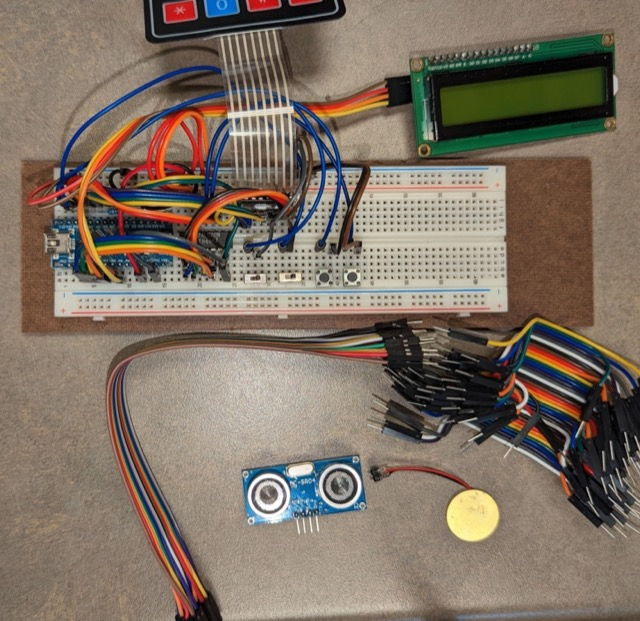
\includegraphics[width=10cm]{hardware/mk1f/components}
    \caption{Components needed for the Range Finder \label{fig:components-mk1f}}
\end{figure}

You will need:
\begin{itemize}
    \item Your Cow Pi hardware circuit
    \item A piezoelectric disc
        \begin{itemize}
            \item Piezoelectric devices can convert electric energy into mechanical energy, and vice-versa
            \item You will use a piezoelectric disc to create an audible alarm
        \end{itemize}
    \item An ultrasonic echo sensor
        \begin{itemize}
            \item The two prominent drums on this device are ultrasonic transducers, one of which converts electricity to 40kHz sound (well above the range of human hearing), and the other of which converts 40kHz sound into electricity
            \item You will measure the time between the ultrasound being transmitted and its reflecting being received to determine the distance to whatever is reflecting the ultrasound
        \end{itemize}
    \item Six male-to-male wires (three of these must be 20cm, and the other three can be 10cm or 20cm)
\end{itemize}

You and your partner only need to modify one of your Cow Pis (but you may modify both).

\subsection{Connecting the Piezoelectric Disc}

The Arduino Nano's pin D13 is used for the Arduino Nano's internal LED, the ``left'' LED.
In the group project, we will use it to control the piezodisc.

\begin{description}
    \checkoffitem{Insert the piezodisc's header into unused rows on the breadboard (Figure~\ref{fig:insertPiezo}).}
    \checkoffitem{Use a 20cm wire to connect the piezodisc's red lead to the Arduino Nano's pin D13 (contact point a1 is a good choice).}
    \checkoffitem{Use another wire to connect the piezodisc's black lead to the upper \ground .}
\end{description}

\begin{figure}
    \centering
    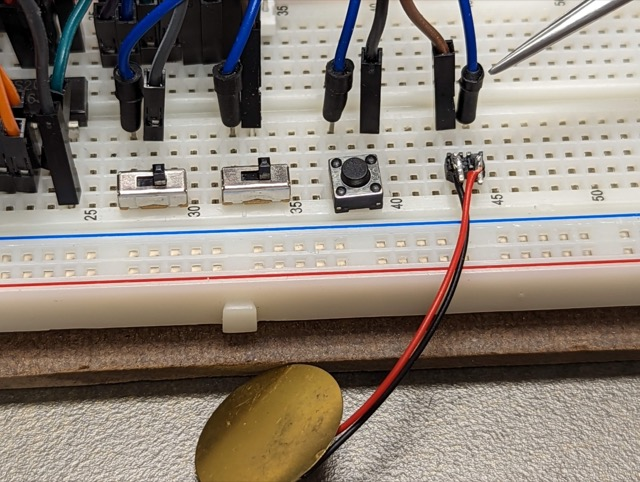
\includegraphics[height=4cm]{hardware/mk1f/adjust_piezo_wire}
    \caption{\label{fig:insertPiezo} Connecting the Piezoelectric Disc.}
\end{figure}

The piezodisc can now be operated through the Arduino Nano's pin D13, which is the pin that the built-in LED is connected to.


\subsection{Connecting the ultrasonic echo sensor}

Take a look at the ultrasonic echo sensor (Figure~\ref{fig:ultrasonic-mk1f}).
Notice that it has four pins, labeled \texttt{Gnd}, \texttt{Echo}, \texttt{Trig}, and \texttt{Vcc}.

\begin{figure}
    \centering
    \subfloat[The back side of the ultrasonic sensor.]{
        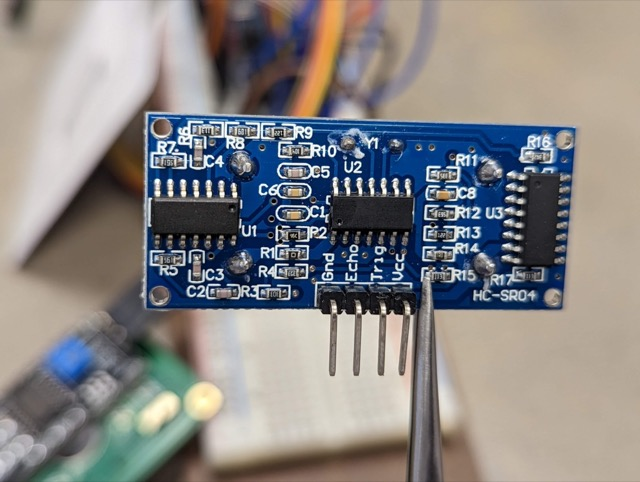
\includegraphics[height=4cm]{hardware/components/ultrasonic_rear}
%        \label{fig:ultrasonicRear}
    }
    \hfil
    \subfloat[The front side of the ultrasonic sensor.]{
        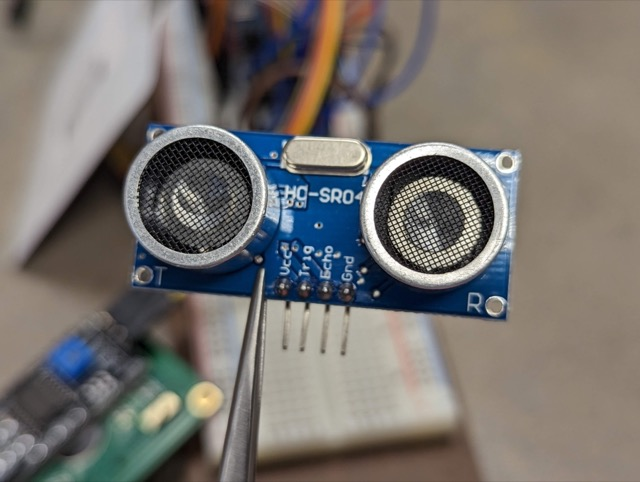
\includegraphics[height=4cm]{hardware/components/ultrasonic_front}
%        \label{fig:ultrasonicFront}
    }
    \caption{The ultrasonic echo sensor. \label{fig:ultrasonic-mk1f}}
\end{figure}

\begin{description}
    \checkoffitem{Insert the ultrasonic echo sensor into unused rows on the breadboard, pointing away from you.
        The ultrasonic transducers should point toward the upper power/ground rails.}
    \checkoffitem{Insert a 20cm wire into contact point j11 (Figure~\ref{fig:insertD2}).
        Make a note of the wire's color for future reference.
        This is your \textbf{D2 wire}.}
    \checkoffitem{Insert a 20cm wire into contact point j10 (Figure~\ref{fig:insertD3}).
        Make a note of the wire's color for future reference.
        This is your \textbf{D3 wire}.}
    \checkoffitem{Insert the D2 wire into the same row as the sensor's \texttt{Trig} pin,
        and the D3 wire into the same row as the sensor's \texttt{Echo} pin (Figure~\ref{fig:ultrasonicD2D3}).}
    \checkoffitem{Use a wire to connect the sensor's \texttt{Gnd} pin to the upper \ground.
        Use another wire to connect the sensor's \texttt{Vcc} pin to the upper \power.
        See Figures~\ref{fig:ultrasonicPwrGnd}--\ref{fig:pwrGnd}.
        For best performance, position these wires so that they are not directly in front of the ultrasonic transducers.}
\end{description}

\begin{figure}
    \centering
    \subfloat[The ultrasonic sensor inserted into the breadboard.]{
        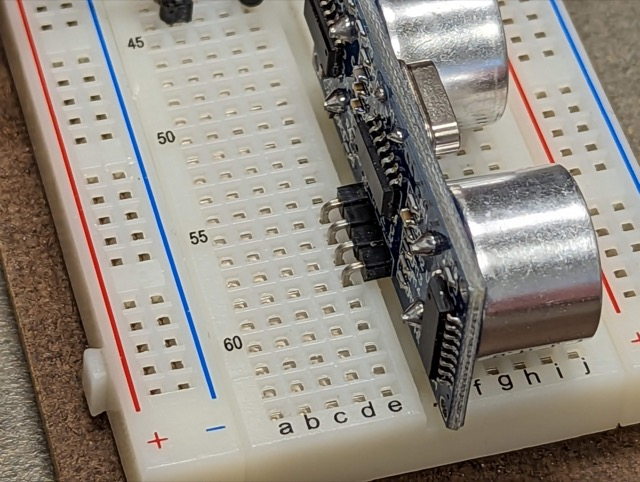
\includegraphics[height=4cm]{hardware/mk1f/ultrasonic_inserted}
        \label{fig:ultrasonicInserted}
    }
    \hfil
    \subfloat[Inserting a wire into contact point j11.]{
        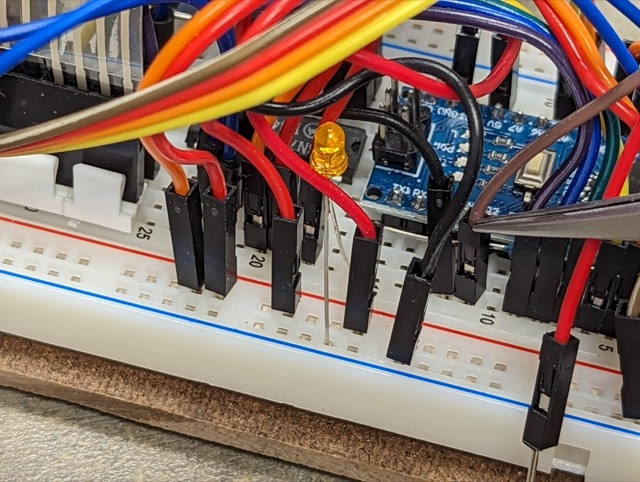
\includegraphics[height=4cm]{hardware/mk1f/insert_D2}
        \label{fig:insertD2}
    }
    \hfil
    \subfloat[Inserting a wire into contact point j10.]{
        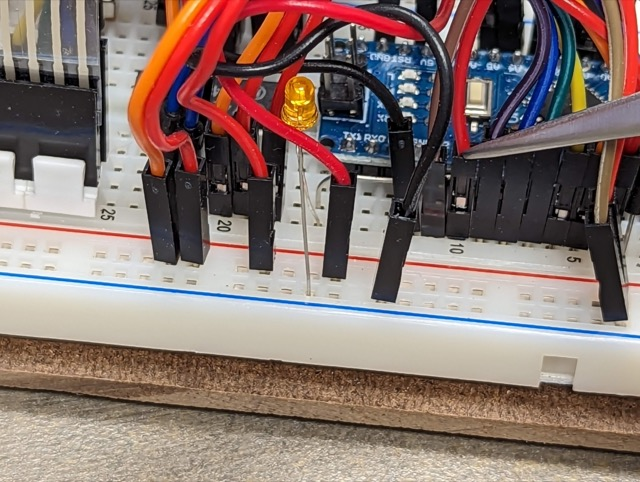
\includegraphics[height=4cm]{hardware/mk1f/insert_D3}
        \label{fig:insertD3}
    }
    \hfil
    \subfloat[The two 20cm wires, ready to be used.]{
        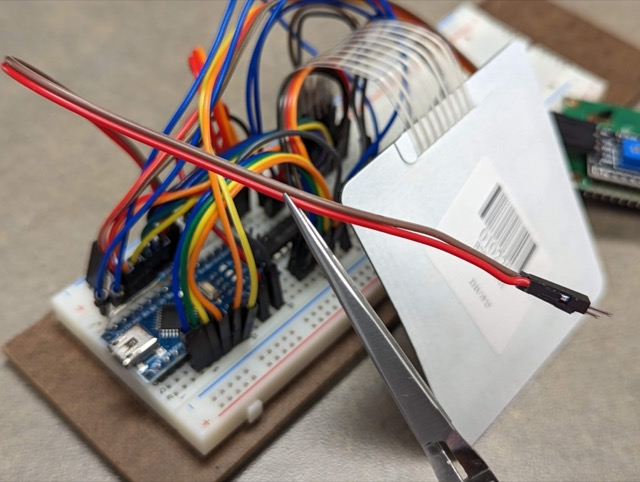
\includegraphics[height=4cm]{hardware/mk1f/20cm_D2_D3}
%        \label{fig:20cmD2D3}
    }
    \hfil
    \subfloat[The ultrasonic sensor connected to the D2 and D3 wires.]{
        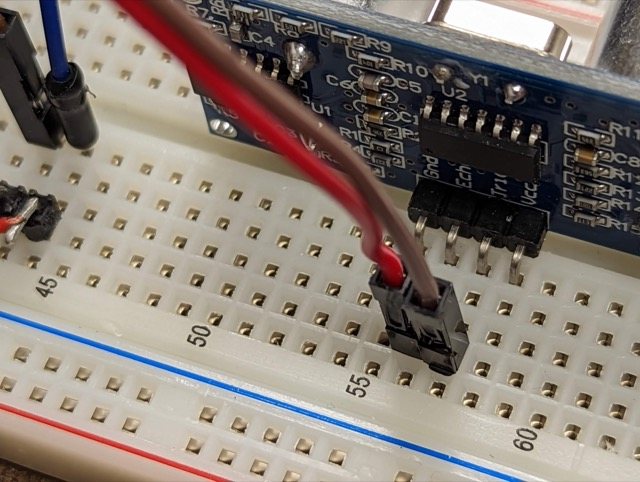
\includegraphics[height=4cm]{hardware/mk1f/ultrasonic_D2_D3}
        \label{fig:ultrasonicD2D3}
    }
    \hfil
    \subfloat[Inserting one end of the power and ground wires.]{
        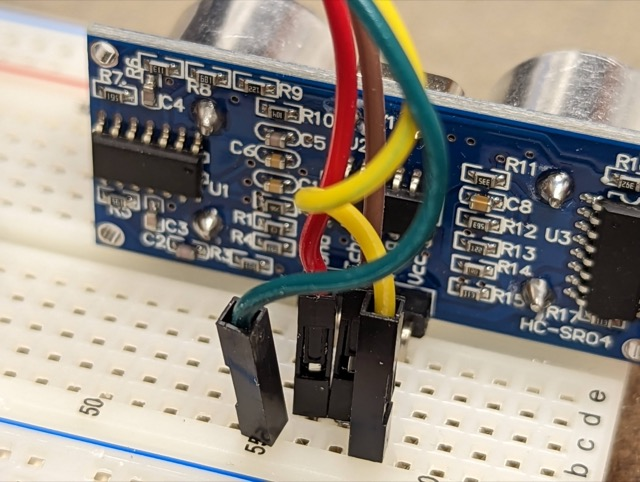
\includegraphics[height=4cm]{hardware/mk1f/ultrasonic_pwr_gnd}
        \label{fig:ultrasonicPwrGnd}
    }
    \hfil
    \subfloat[Inserting the other end of the power and ground wires in the power and ground rails.]{
        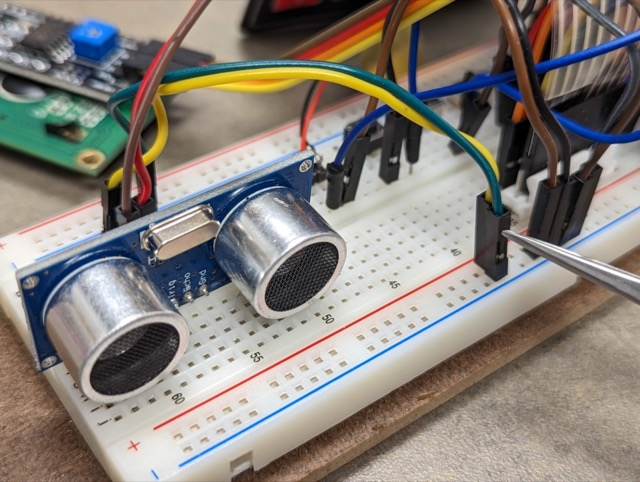
\includegraphics[height=4cm]{hardware/mk1f/pwr_gnd}
        \label{fig:pwrGnd}
    }
    \caption{Connecting the ultrasonic echo sensor.}
\end{figure}

The ultrasonic echo sensor is now connected to the Arduino Nano's pins D2 \& D3.
The starter code will configure D2 (\lstinline{TRIGGER}) to be an output pin and D3 (\lstinline{ECHO}) to be an input pin.

%\begin{figure}
%    \centering
%    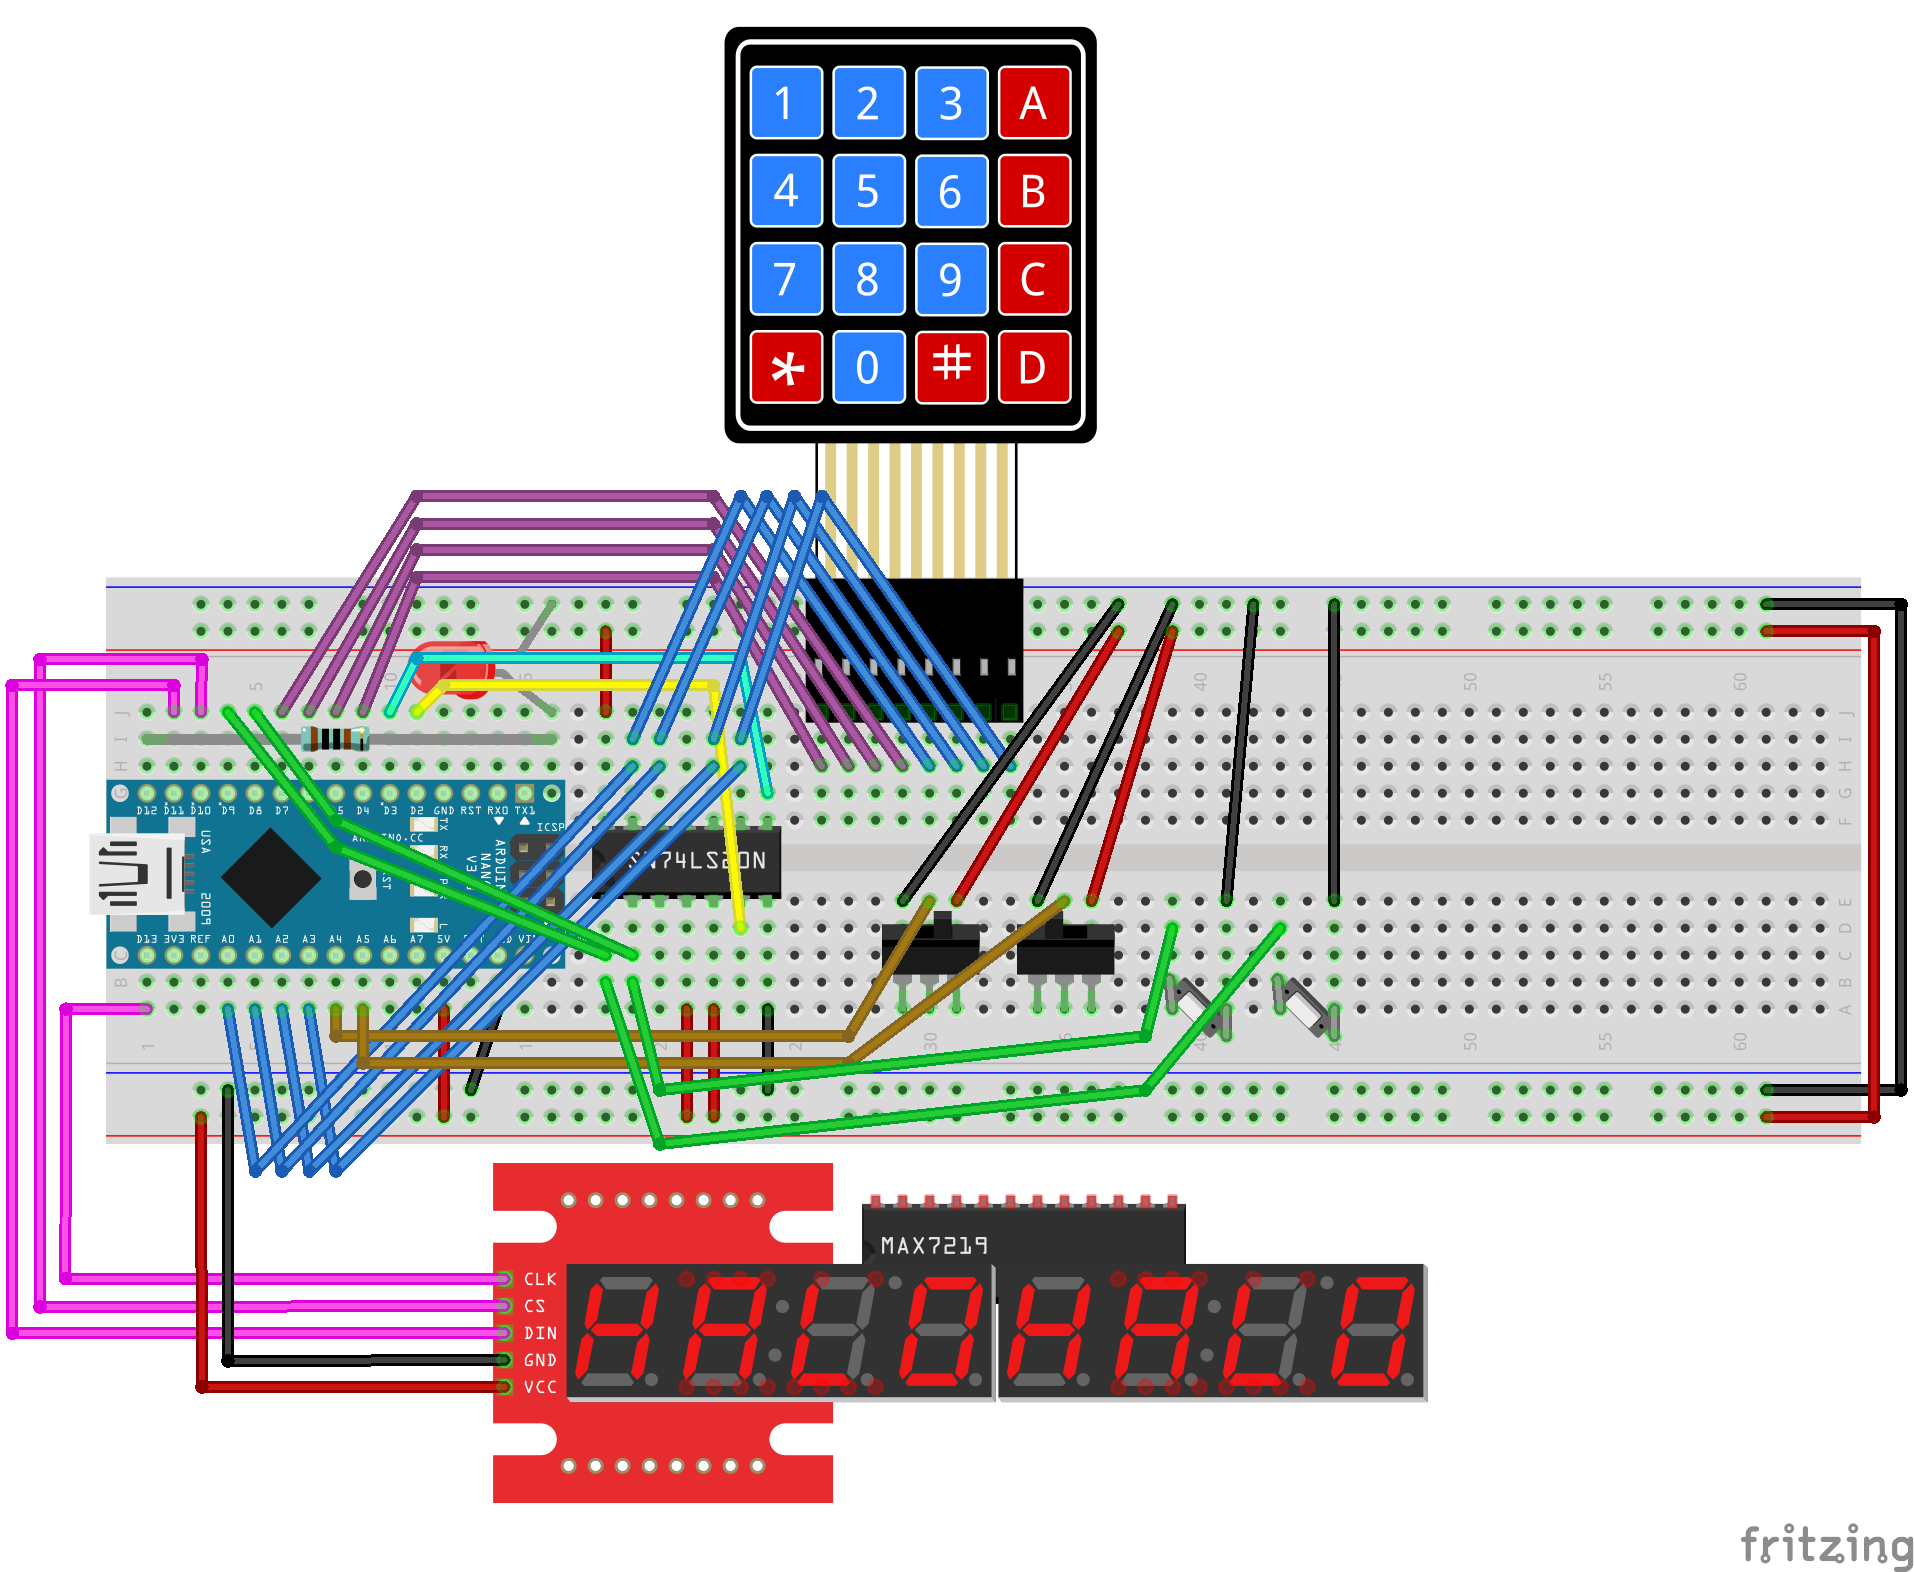
\includegraphics[width=10cm]{hardware/complete}
%    \caption{The Cow Pi circuit with modfications complete.}
%\end{figure}

\vspace{1cm}

Your Cow Pi circuit is now ready for you to design and code the software for a range finder and alarm.
